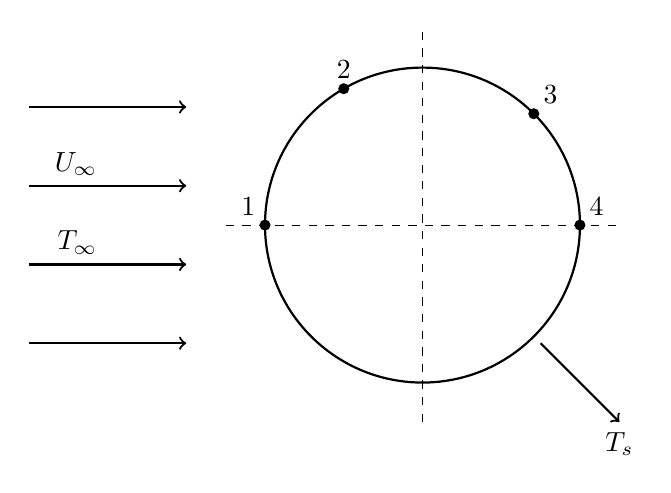
\begin{tikzpicture}
    % Draw the circle
    \draw[thick] (0,0) circle(2);

    % Draw the dots on the circle with labels
    \fill (2,0) circle(2pt) node[above right] {4};
    \fill (-2,0) circle(2pt) node[above left] {1};
    \fill (-1,1.732) circle(2pt) node[above] {2};
    \fill (1.414,1.414) circle(2pt) node[above right] {3};

    % Draw center dashed lines
    \draw[dashed] (-2.5,0) -- (2.5,0); % Horizontal
    \draw[dashed] (0,-2.5) -- (0,2.5); % Vertical

    % Draw the arrow with T_s label
    \draw[->, thick] (1.5,-1.5) -- (2.5,-2.5) node[below] {$T_s$};

    % Draw flow lines on the left side with labels
    \draw[->, thick] (-5, 1.5) -- (-3, 1.5);
    \draw[->, thick] (-5, 0.5) -- (-3, 0.5) node[midway, above left] {$U_\infty$};
    \draw[->, thick] (-5, -0.5) -- (-3, -0.5) node[midway, above left] {$T_\infty$};
    \draw[->, thick] (-5, -1.5) -- (-3, -1.5);
\end{tikzpicture}
